
\documentclass{jtetiproposalskripsi}

%-----------------------------------------------------------------
%Disini awal masukan untuk data proposal skripsi
%-----------------------------------------------------------------
\titleind{SISTEM INFORMASI PEMESANAN BAJU KONVEKSI UD.CANTIK COLLECTION}
\fullname{RISKY SUPRAYOGI}

\idnum{1200631016}

\approvaldate{13 Januari 2015}

\degree{Sarjana Teknik Elektro}

\yearsubmit{2015}

\program{Manajemen Informatika}

\headprogram{Sarjiya, S.T., M.T., Ph.D.}

\dept{Manajemen Informatika }

\firstsupervisor{Bakhtiyar Hadi P. S.Kom}
\firstnip{12 03 716}




%-----------------------------------------------------------------
%Disini akhir masukan untuk data proposal skripsi
%-----------------------------------------------------------------

\begin{document}

\cover

\approvalpage

%-----------------------------------------------------------------
%Disini akhir masukan untuk muka skripsi
%-----------------------------------------------------------------

%-----------------------------------------------------------------
%Disini awal masukan Intisari
%-----------------------------------------------------------------
\begin{abstractind}
Abstract : Dewasa ini teknologi pengetahuan teknologi semakin meningkat demi pembangunan yang lebih maju, banyak took online yang memakai suatu website untuk memperluas pemasaran produk mereka, tetapi tidak semua UD (Usaha Dagang) memakai cara ini dikarenakan masih banyaknya para wiraswasta yang masih kurang pengetahuan terhadap teknologi computer. Pembuatan rancangan website ini bertujuan agar pemasaran UD. CANTIK COLLECTION mempermudah dalam memasarkan barang dengan cara mepostingnya di website ini, lebih menunjang perkembangan pemasaran pakaian karena saat ini pemasarannya hanya sebatas lingkup Kecamatan, mempermudah calon pembeli untuk melihat barang tanpa harus repot - repot datang ke UD tersebut. Pembuatan perancangan  website ini menggunakan aplikasi dreamweaver sebagai editornya, template website sebagai tampilan websitenya, MySQL sebagai database, Xampp sebagai server. Oleh karenanya pembuatan rancangan website untuk UD. CANTIK COLLECTION sangat membantu dalam hal pemasaran yang akan berdampak meluasnya pemasaran pakaiannya.

\bigskip
\textbf{Kata kunci} : Website UD. Cantik Collection, Dreamweaver, Template, MySQL, Xampp.
\end{abstractind}
%-----------------------------------------------------------------
%Disini akhir masukan Intisari
%-----------------------------------------------------------------

\tableofcontents
\addcontentsline{toc}{chapter}{DAFTAR ISI}
\selectlanguage{bahasa}\clearpage\pagenumbering{arabic}\setcounter{page}{1}

%-----------------------------------------------------------------
%Disini awal masukan untuk Bab
%-----------------------------------------------------------------
\chapter{PENDAHULUAN}

\section{Latar Belakang Masalah}
Perkembangan dunia saat ini sangat dipengaruhi oleh perkembangan teknologi informasi yang memungkinkan terjadinya perpindahan data informasi yang sangat cepat. Hal ini menuntut setiap individu ataupun institusi untuk terus mengikuti perkembangan teknologi informasi. Salah satu teknologi informasi yang sangat berkembang saat ini adalah Web Programming. Seiring dengan kemajuan dunia ilmu pengetahuan dan teknologi, terutama pada teknologi komputer maka kebutuhan terhadap informasi yang cepat dan akurat juga ikut berkembang. Komputer merupakan pemroses data yang cepat dan akurat didukung dengan berbagai macam pemrograman yang ada dalam menyajikan informasi terutama di bidang pemrograman yang berbasis internet. 

Perusahaan kecil maupun yang sudah berkembang sangat membutuhkan suatu sistem untuk mempermudah operasional suatu perusahaan agar perusahaan tersebut mampu berkembang maju dan bersaing dengan perusahaan lain. Kemudahan yang dapat diperoleh adalah kemudahan mengakses data, mengisi data perusahaan maupun dalam pembuatan laporan keuangan maupun laporan pemesanan dari barang perusahaan tersebut. Ketika suatu perusahaan masih belum memiliki sistem informasi ini maka dalam kegiatan operasionalnya masih memiliki resiko kesalahan penginputan maupun pembuatan laporan. Oleh karena itu sistem informasi ini sangat penting demi menunjang kesuksesan perusahaan tersebut.

Perusahaan yang masih berkembang seperti UD Cantik Collection yang bertempat di Kecamatan Bangorejo Kabupaten Banyuwangi memiliki masalah dalam penginputan pemesanan baju konveksi, selain membutuhkan waktu yang lama, media penyimpanan yang rentan rusak seperti pada kertas, dan pembuatan arsip laporan keuangan setiap bulan yang menggunakan cara manual yaitu cara tulis tangan memiliki resiko kesalahan yang lebih tinggi, yang dapat menghambat perkembangan perusahaan tersebut. Dengan demikian maka UD Cantik Collection ini membutuhkan suatu aplikasi untuk menyimpan data tentang pemesanan dan pembayaran dalam kegiatan operasional sehari – hari. 

Dari uraian diatas, penulis bermaksud untuk membuat sebuah aplikasi yang bermanfaat bagi  UD Cantik Collection dalam menangani masalah ini, yaitu dengan membuat sebuah \textbf{ Sistem Informasi Pemesanan Baju Konveksi UD Cantik Collection}.

\section{Rumusan Masalah}
Berdasarkan latar belakang yang telah diuraikan di atas maka didapatkan beberapa rumusan masalah sebagai berikut :
\begin{itemize}
\item[1.]	Bagaimana merancang sebuah sistem informasi pemesanan baju konveksi  yang dapat di gunakan user untuk pelangan pemesanan baru.
\item[2.]	Bagaimana membangun sistem informasi pemesanan baju konveksi ini agar mampu memberikan informasi kepada user dalam pengisian data laporan keuangan dan sekaligus memberikan kemudahan bagi UD Cantik Collection dalam pengisian pelanggan yang memesan baju secara efektif dan efisien. 


\end{itemize}

\section{Batasan Masalah}
Untuk menyelesaikan masalah diatas diberikan batasan masalah sebagai berikut :
\begin{itemize}
\item[1.]Aplikasi dibangung hanya untuk mengatur pemesanan baju konveksi
\item[2.]Pembuatan rekap laporan keuangan untuk data pemesanan baju konveksi UD Cantik Collection.

\end{itemize}


\section{Tujuan Penelitian}
Tujuan dari pembuatan sistem ini adalah :
\begin{itemize}
\item[1.]Merancang pembuatan Sistem Informasi Pemesanan Baju Konveksi
\item[2.]Membangun Sistem Informasi Pemesanan Baju Konveksi untuk mempermudah dalam pengisian data pelanggan yang memesan baju sekaligus memberikan laporan data pemesanan.

\end{itemize}


\section{Manfaat Penelitian}
Manfaat dari sistem ini adalah :
\begin{itemize}
\item[1.]Memberikan kemudahan pengisian data bagi user untuk proses pemesanan baju.
\item[2.]Mempercepat proses pengisian data pemesanan dan mempercepat proses rekap laporan pemesanan.
\item[3.]Memberikan kebutuhan  informasi untuk pemilik UD Cantik Collection tentang laporan yang diterima menggunakan sistem informasi ini.
\end{itemize}


%-------------------------------------------------------------------------------
\chapter{LANDASAN TEORI}          
\section{Landasan Teori}      
\subsection{Pengertian Sistem}
Suatu sistem sangatlah dibutuhkan dalam suatu perusahaan atau instansi pemerintahan, karena sistem sangatlah menunjang terhadap kinerja perusahaan atau instansi pemerintah, baik yang berskala kecil maupun besar. Supaya dapat berjalan dengan baik diperlukan kerjasama diantara unsure-unsur yang terkait dalam sistem tersebut. Sistem adalah sekumpulan unsur / elemen yang saling berkaitan dan saling mempengaruhi dalam melakukan kegiatan bersama untuk mencapai suatu tujuan. Jadi, secara umum Pengertian Sistem adalah perangkat unsur yang teratur saling berkaitan sehingga membentuk suatu totalitas.

Sistem adalah suatu jaringan kerja dari prosedur-prosedur yang saling berhubungan , berkumpul bersama-sama untuk melakukan suatu kegiatan atau untuk menyelesaikan suatu sasaran yang tertentu.(Jogiyanto,2005,1).  Pengertian lain dari sistem adalah:  Sistem adalah suatu urutan-urutan yang tepat dari  tahapan-tahapan instruksi yang menerangkan apa yang harus dikerjakan, siapa yang mengerjakan, kapan  dikerjakan, dan bagaimana mengerjakannya. (Al-Bahra Bin Ladjamudin ,2005:3)

Berdasarkan pengertian di atas penulis menyimpulkan sistem adalah sekumpulan prosedur atau tahapan yang saling  berhubungan untuk mencapai sebuah tujuan tertentu

\subsection{Pengertian Infromasi}
Dalam manajemen, informasi merupakan data yang telah diproses sehingga mempunyai arti tertentu bagi penerimanya.Sumber dari informasi adalah Data, sedangkan Data itu sendiri adalah Kenyataan yang menggambarkanm suatu kejadian, sedangkan kejadian itu merupakan suatu peristiwa yang terjadi pada waktu tertentu .dalam hal ini informasi dan data saling berkaitan.

Informasi  adalah Data yang diolah menjadi bentuk yang lebih berguna dan lebih berarti bagi yang menerimanya. (Jogiyanto,2005; 8). Pengertian lain tentang   informasi adalah informasi adalah data yang telah  diolah  menjadi bentuk yang lebih berarti dan berguna bagi  penerimanya untuk mengambil keputusan msa kini maupun  yang akan datang. (Al-Bahra Bin Ladjamudin ,2005:8) 

\subsection{Pengertian Sistem Informasi}
Sistem informasi adalah; Sistem informasi adalah sistem yang diciptakan oleh para analisis dan manajer guna melaksanakan tugas khusus tertentu yang sangat esensial bagi berfungsinya organisasi’ (George M.Scott,2001;4) Sedangan sistem informasi menurut Jogianto dalam  bukunya yang berjudul  Analisis dan Desain Sistem Informasi adalah:  Sistem informasi adalah suatu sistem di dalam suatu  organisasi yang mempertemukan kebutuhan pengolahan  transaksi harian, mendukung operasi, bersifat manajerial dan kegiatan strategi dari suatu organisasi dan menyedi akan pihak  luar tertentu dengan laporan–laporan yang  diperlukan.( Jogiyanto, 2005:11) 

\subsection{Website}
World Wide Web atau WWW atau juga dikenal dengan WEB adalah salah satu layanan yang didapat oleh pemakai computer yang terhubung ke internet. Web ini menyediakan informasi bagi pemakai computer yang terhubung ke internet dari sekedar informasi “sampah” atau informasi yang tidak berguna sama sekali sampai informasi yang serius; dari informasi yang gratisan sampai informasi yang komersial. Website atau situs dapat diartikan sebagai kumpulan halaman-halaman yang digunakan untuk menampilkan informasi teks, gambar diam atau gerak, animasi, suara, dan atau gabungan dari semuanya itu baik yang bersifat statis maupun dinamis yang membentuk satu rangkaian bangunan yang saling terkait dimana masing-masing dihubungkan dengan jaringan-jaringan halaman (hyperlink).

Menurut Suwanto Raharjo S.Si, M.Kom, Web merupakan salah satu layanan internet yang paling banyak digunakan dibanding dengan layanan lain seperti ftp, gopher, news atau bahkan email. Sedangkan menurut Wahana Komputer, Web adalah formulir komunikasi interaktif yang digunakan pada sutu jaringan komputer. 

\subsection{Unsur-Unsur Website atau Situs}
Untuk menyediakan keberadaan sebuah website, maka harus tersedia unsur-unsur penunjangnya, adalah sebagai berikut:
\begin{itemize}
\item[1)]Nama domain (Domain name/URL - Uniform Resource Locator)

Pengertian Nama domain atau biasa disebut dengan Domain Name atau URL adalah alamat unik di dunia internet yang digunakan untuk mengidentifikasi sebuah website, atau dengan kata lain domain name adalah alamat yang digunakan untuk menemukan sebuah website pada dunia internet. Contohnya adalah http://www.baliorange.net http://www.detik.com
Nama domain diperjualbelikan secara bebas di internet dengan status sewa tahunan. Nama domain sendiri mempunyai identifikasi ekstensi/akhiran sesuai dengan kepentingan dan lokasi keberadaan website tersebut.

\item[2)]Rumah tempat website (Web hosting) 

Pengertian Web Hosting dapat diartikan sebagai ruangan yang terdapat dalam harddisk tempat menyimpan berbagai data, file-file, gambar dan lain sebagainya yang akan ditampilkan di website. Besarnya data yang bisa dimasukkan tergantung dari besarnya web hosting yang disewa/dipunyai, semakin besar web hosting semakin besar pula data yang dapat dimasukkan dan ditampilkan dalam website. Web Hosting juga diperoleh dengan menyewa. 

\item[3)]Bahasa Program (Scripts Program)  

Adalah bahasa yang digunakan untuk menerjemahkan setiap perintah dalam website yang pada saat diakses. Jenis bahasa program sangat menentukan statis, dinamis atau interaktifnya sebuah website. Semakin banyak ragam bahasa program yang digunakan maka akan terlihat website semakin dinamis, dan interaktif serta terlihat bagus. Beragam bahasa program saat ini telah hadir untuk mendukung kualitas website. Jenis jenis bahasa program yang banyak dipakai para desainer website antara lain HTML, ASP, PHP, JSP, Java Scripts, Java applets dsb. 

\item[4)]Desain website

Setelah melakukan penyewaan domain name dan web hosting serta penguasaan bahasa program (scripts program), unsur website yang penting dan utama adalah desain. Desain website menentukan kualitas dan keindahan sebuah website. Desain sangat berpengaruh kepada penilaian pengunjung akan bagus tidaknya sebuah website. Untuk membuat website biasanya dapat dilakukan sendiri atau menyewa jasa website designer. 
\end{itemize}


\subsection{Fungsi Web }
Secara umum situs web mempunyai fungsi sebagai berikut:

\begin{itemize}
\item[1.] Fungsi komunikasi 

Situs web yang mempunyai fungsi komunikasi pada umumnya adalah situs web dinamis. Karena dibuat menggunakan pemograman web (server side) maka dilengkapi fasilitas yang memberikan fungsi-fungsi komunikasi, seperti web mail, form contact, chatting form, dan yang lainnya.


\item[2.] Fungsi informasi  

Situs web yang memiliki fungsi informasi pada umumnya lebih menekankan pada kualitas bagian kontennya, karena tujuan situs tersebut adalah menyampaikan isisnya. Situs ini sebaiknya berisi teks dan grafik yang dapat di download dengan cepat. Pembatasan penggunaan animasi gambar dan elemen bergerak seperti shockwave dan java diyakini sebagai langkah yang tepat, diganti dengan fasilitas yang memberikan fungsi informasi seperti news, profile company, library, reference,dll.

\item[3.]Fungsi entertainment 

Situs web juga dapat memiliki fungsi entertainment/hiburan. Bila situs web kita berfungsi sebagai sarana hiburan maka penggunaan animasi gambar dan elemen bergerak dapat meningkatkan mutu presentasi desainnya, meski tetap harus mempertimbangkan kecepatan downloadnya.

\item[4.] Fungsi transaksi 

Situs web dapat dijadikan sarana transaksi biisnis, baik barang, jasa, atau lainnya. Situs web ini menghubungkan perusahaan, konsumen, dan komunitas tertentu melalui transaksi elektronik. Pembayarannya bisa menggunakan kartu kredit, transfer, atau dengan membayar secara langsung.

\end{itemize}

\subsection{Xampp}
XAMPP adalah sebuah software web server apache yang didalamnya sudah tersedia database server mysql dan support php programming. XAMPP merupakan software yang mudah digunakan, gratis dan mendukung instalasi di Linux dan Windows
 XAMPP adalah sebuah software yang berfungsi untuk menjalankan website berbasis PHP dan menggunakan pengolah data MySQL dikomputer local”.  XAMPP berperan sebagai server web pada komputer anda. XAMPP juga dapat disebut sebuah CPanel server virtual, yang dapat membantu anda melakukan preview sehingga dapat memodifikasi website tanpa harus online atau terakses dengan internet (Yogi wicaksono, 2008:7).

Berikut adalah 4 komponen penting didalam xampp :

\begin{itemize}
\item[1.]Apache

Apache adalah sebuah nama web server yang bertanggung jawab pada request-response HTTP dan logging informasi secara detail(kegunaan basicnya). Selain itu, Apache juga diartikan sebagai suatu web server yang kompak, modular, mengikuti standar protokol HTTP, dan tentu saja sangat digemari. Kesimpulan ini bisa didapatkan dari jumlah pengguna yang jauh melebihi para pesaingnya. Sesuai hasil survai yang dilakukan oleh Netcraft, bulan Januari 2005 saja jumlahnya tidak kurang dari 68% pangsa web server yang berjalan di Internet. Ini berarti jika semua web server selain Apache digabung, masih belum bisa mengalahkan jumlah Apache.

Apache memiliki fitur-fitur canggih seperti pesan kesalahan yang dapat dikonfigur, autentikasi berbasis basis data dan lain-lain. Apache juga didukung oleh sejumlah antarmuka pengguna berbasis grafik (GUI) yang memungkinkan penanganan server menjadi mudah. Apache merupakan perangkat lunak sumber terbuka dikembangkan oleh komunitas terbuka yang terdiri dari pengembang-pengembang dibawah naungan Apache Software Foundation.

Saat ini ada dua versi Apache yang bisa dipakai untuk server produksi, yaitu versi mayor 2.0 dan versi mayor 1.3. Apache merupakan webserver yang paling banyak digunakan saat ini. Hal ini disebabkan oleh beberapa sebab, di antaranya adalah karena sifatnya yang opensource dan mudahnya mengkostumisasikannya. diantaranya dengan menambahkan support secure protocol melalui ssl dan konektifitasnya dengan database server melalui bahasa scripting PHP .


\item[2.] PHP 

PHP adalah bahasa pemrograman script server-side yang didesain untuk pengembangan web, tetapi juga bisa digunakan sebagai bahasa pemrograman umum (wikipedia). PHP pertama kali  di kembangkan pada tahun 1995 oleh Rasmus Lerdorf, namun sekarang dikelola oleh The PHP Group. Situs resmi PHP beralamat di http://www.php.net. Untuk mengawali kode dalam PHP menggunakan kode <? Dan diakhiri tanda ?>.
Definisi PHP menurut  Kasiman peranginangin dalam bukunya yang berjudul Aplikasi Web  dengan PHP dan MySQLmenjelaskan bahwa “PHP  singkatan dari Hypertext Preprocessor yang di gunakan sebagai bahasa scrip server-side dalam pengembangan web yang disisipkan pada  dokumen HTML”  (Kasiman, 2006:2)  Definisi lain dari PHP  “php adalah script yang digunakan untuk membuat halaman website yang dinamis”  (Anhar , 2010:03) 
Berikut adalah  kelebihan Bahasa Pemrograman PHP dibandingkan dengan Bahasa Pemrograman Komputer yang lain, Diantaranya sebagai berikut :
\begin{itemize}
\item[a.]Sangat Banyak Server-server website yang mendukung bahasa pemrograman PHP ini karena fungsinya yang bagus.
\item[b.] Bahasa Pemrograman PHP dapat digunakan dengan mudah oleh setiap Web Developer dikarenakan script dan kode-kode Bahasa PHP ini sangat mudah dipahami.
\item[c.] PHP adalah Bahasa Pemrograman Komputer yang sering dan memiliki banyak refrensi dari segala sumber.
\item[d.] Bahasa Pemrograman PHP Bersifat Sumber Terbuka yaitu dapat digunakan di segala jenis mesin Seperti Unix, Windows, Linux, DLL.
\item[e.]Bahasa Pemrograman PHP Dapat menjalankan sebuah ataupun beberapa perintah dari suatu sistem.
\item[f.]PHP dapat dijalankan dan digunakan secara runtime melalui sebuah konsol.
\end{itemize}


\item[3.]Fungsi entertainment 

Situs web juga dapat memiliki fungsi entertainment/hiburan. Bila situs web kita berfungsi sebagai sarana hiburan maka penggunaan animasi gambar dan elemen bergerak dapat meningkatkan mutu presentasi desainnya, meski tetap harus mempertimbangkan kecepatan downloadnya.

\item[4.] Fungsi transaksi 

Situs web dapat dijadikan sarana transaksi biisnis, baik barang, jasa, atau lainnya. Situs web ini menghubungkan perusahaan, konsumen, dan komunitas tertentu melalui transaksi elektronik. Pembayarannya bisa menggunakan kartu kredit, transfer, atau dengan membayar secara langsung.

\end{itemize}

\subsection{MySQL}
MySQL adalah sebuah implementasi dari sistem manajemen basisdata relasional (RDBMS) yang didistribusikan secara gratis. Setiap pengguna dapat secara bebas menggunakan MySQL, namun dengan batasan perangkat lunak tersebut tidak boleh dijadikan produk turunan yang bersifat komersial. MySQL sebenarnya merupakan turunan salah satu konsep utama dalam basisdata yang telah ada sebelumnya; SQL (Structured Query Language). SQL adalah sebuah konsep pengoperasian basisdata, terutama untuk pemilihan atau seleksi dan pemasukan data, yang memungkinkan pengoperasian data dikerjakan dengan mudah secara otomatis. Kehandalan suatu sistem basisdata (DBMS) dapat diketahui dari cara kerja pengoptimasi-nya dalam melakukan proses perintah-perintah SQL yang dibuat oleh pengguna maupun program-program aplikasi yang memanfaatkannya. Sebagai peladen basis data, MySQL mendukung operasi basisdata transaksional maupun operasi basisdata non-transaksional. Pada modus operasi non-transaksional, MySQL dapat dikatakan unggul dalam hal unjuk kerja dibandingkan perangkat lunak peladen basisdata kompetitor lainnya.

Definisi MySQL menurut  pakar ahli menjelaskan bahwa mysql merupakan software yang tergolong database server dan bersifat  open source  (Abdul Kadir 2009:15)


\subsection{PHPMyAdmin }

PhpMyAdmin adalah sebuah aplikasi web yang ditulis menggunakan bahasa pemrograman PHP. Sebagaimana aplikasi-aplikasi lain untuk lingkungan web (aplikasi yang dibuka menggunakan peramban atau browser), phpMyAdmin juga mengandung unsur HTML/XHTML, CSS, dan juga kode JavaScript. Aplikasi web ini ditujukan untuk memudahkan pengelolaan basis data MySQL dengan penyajian tampilan web (user interface) yang lengkap . 

PhpMyAdmin merupakan aplikasi web yang bersifat open souce (sumber terbuka) sejak pertama kali dibuat dan dikembangkan. Dengan dukungan dari banyak developer dan translator, aplikasi web phpMyAdmin mengalami perkembangan yang cukup pesat dengan ketersediaan banyak pilihan bahasa. Sampai saat ini, ada kurang lebih 65 bahasa yang didukung oleh aplikasi web phpMyAdmin.

PhpMyAdmin menawarkan fitur yang mencangkup pengelolaan keseluruhan server MySQL (memerlukan super-user) dan juga basis data tunggal. phpMyAdmin juga mempunyai sistem internal yang digunakan untuk mengelola metadata dan mendukung fitur-fitur untuk operasi tingkat lanjut.


\subsection{Pengertian Konveksi }

Industri konveksi adalah suatu perusahaan yang menghasilkan pakaian jadi  pakaian wanita, pria, anak, pakaian olahraga, maupun pakaian-pakaian partai politik. Industri konveksi bisa di bilang perusahaan yang sedang karena tenaga kerjanya masih dibilang sedikit. Umumnya, perusahaan-perusahaan konveksi mempergunakan bahan baku berupa tekstil dari bermacam-macam jenis, seperti katun, kaos, linen, polyester, rayon, dan bahan-bahan syntesis lain ataupun campuran dari jenis bahan-bahan tersebut.



%-------------------------------------------------------------------------------
\chapter{METODOLOGI PENELITIAN}

\section{Flowchart Metode Penelitian}

\begin{table}[ht!]
  \centering
    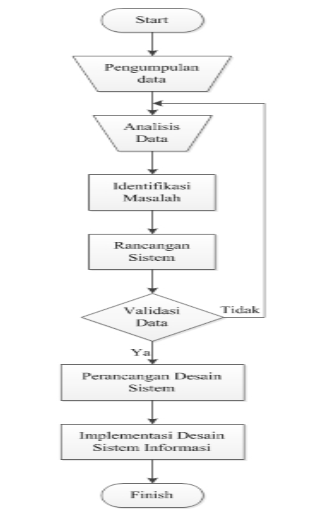
\includegraphics[width=0.6\textwidth]{gambar/FC}
    \caption{Flowchart Penelitian}
    \label{wsn}
\end{table}
\newpage

\begin{itemize}
\item[1.]Pengumpulan Data

Didalam penelitian ini penulis mengawali kegiatan dengan pengumpulan data dari UD. Cantik Collection sebagai bahan pembuatan rancangan dari sistem informasi yang akan penulis buat. Pegumpulan data ini dengan cara kuisioner yang memberikan pertanyaan tertulis yang akan dijawab oleh narasumber, sedangkan cara yang kedua yaitu dengan cara wawancara langsung kepada narasumber dengan memberikan pertanyaan – pertanyaan yang akan dijawab oleh narasumber.

\item[2.] Analisis Data

Proses kedua yaitu analisis data, proses ini bertujuan untuk menganalisis data yang telah dikumpulkan oleh penulis setelah melalui proses pengumpulan data.

\item[3.]Identifikasi Masalah

Setelah penulis menganalisis data barulah penulis mencari permasalahan dari sistem yang ada di UD. Cantik Collection,proses identifikasi masalah inilah yang kemudian akan dibuat suatu rancangan sistem untuk mengatasi masalah dalam sistem yang lama.
\item[d.] Bahasa Pemrograman PHP Bersifat Sumber Terbuka yaitu dapat digunakan di segala jenis mesin Seperti Unix, Windows, Linux, DLL.

\item[4.]Rancangan Sistem
Proses rancangan sistem ini penulis memulai pembuatan rancangan sistem mengenai data yang telah penulis kumpulkan dan masalah apa saja yang ada di sistem yang lama.

\item[5.]Validasi Data

Didalam proses validasi data ini, penulis meneliti kembali rancangan dari sistem, apabila masih ada kekurangan didalam sistem yang baru maka akan kembali ke proses analisis data untuk menganalisis data kembali, apabila data yang ada di rancangan sistem sudah terpenuhi maka masuk ke proses selanjutnya yaitu perancangan desain sistem.

\item[6.]Perancangan Desain Sistem

Proses perancangan desain sistem ini penulis membuat sebuah desain sistem setelah semua data yang penulis kumpulkan sudah valid atau terpenuhi. sebagai desain sistem untuk mengatasi permasalahan yang ada di UD. Cantik Collection.

\item[7.]Implementasi Desain Sistem Informasi

Proses ini menerapkan desain sistem dan kemudian mengimplementasikannya ke sistem yang baru.

\end{itemize}

\section{Prosedur Penelitian}
\subsection{Studi Pustaka}

Melakukan studi pustaka untuk pengumpulan data dengan cara mengadakan studi penelaahan terhadap buku-buku, litertur-literatur, catatan-catatan, dan laporan-laporan yang ada hubungannya dengan masalah yang dipecahkan Sehingga dengan informasi – informasi tersebut dapat digunakan sebagai acuan dalam penyelesaian masalah yang ada didalam sistem lama.

\subsection{Studi Pustaka}

Data primer diperoleh dengan cara :
\begin{itemize}
\item[1.]Kiesioner

Mengajukan tertulis kepada responden atau narasumber. Jawaban responden atas semua pertanyaan dalam kuesioner kemudian dicatat sebagai data.

\item[2.]Observasi

Mengamati secara langsung di tempat UD. CAntik Collection yang kemudian ditulis sebagai bahan atau data. Wawancara

\item[3.] Wawancara

Pengambilan data melalui wawancara /secara lisan langsung dengan narasumber. Jawaban responden atau narasumber tersebut kemudian dirangkum oleh penulis. 
\end{itemize}

Sedangkan data sekunder diperoleh dengan cara :

\begin{itemize}
\item[1.]Studi dokumentasi

Studi dokumentasi digunakan untuk mencari data-data sekunder yang dibutuhkan dalam melakukan tata kelola keuangan yang ada.

\item[2.]Akses internet

Akses internet digunakan untuk mencari data pendukung dari berbagai buku,ebook,maupun jurnal-jurnal yang relevan yang terpercaya.
\end{itemize}

\section{Alat Bantu}

Untuk mempermudah dalam penelitian ini, penulis memiliki alat bantu antara lain :

\section{Jadwal Kegiatan}
Penelitian direncanakan akan dilaksanakan selama 6 bulan . Rincian rencana jadwal penelitian dicantumkan dalam tabel berikut.

\subsection{Perangkat Keras yaitu }

\begin{itemize}
\item[1.]Prosesor Intel Core i3

\item[2.] Memori 4 GB

\item[3.] Harddisk 500 GB
\end{itemize}
\subsection{Perangkat Lunak yaitu }
\begin{itemize}
\item[1.]Microsoft Windows 7 

\item[2.]Notepad++

\item[3.]Dreamweaver

\item[4.]MySQL
\end{itemize}

\section{Jadwal Penelitian}

Untuk melakukan penelitian ini, penulis membuat jadwal penelitian agar dapat selesai tepat waktu yang telah direncanakan. Jadwal penelitian tersebut adalah sebagai berikut :

\begin{center}
Tabel 3.1. Jadwal Penelitian.
\end{center}
\vspace{-0.5cm}
\begin{figure}[ht!]
  \centering
    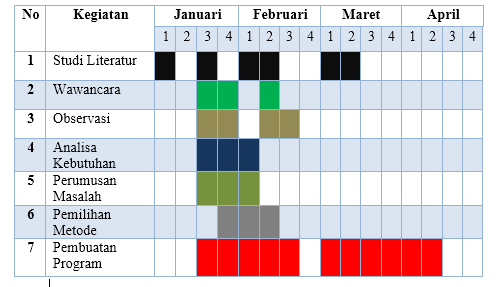
\includegraphics[width=1\textwidth]{gambar/jadwal}
\end{figure}

%-----------------------------------------------------------------
%Disini akhir masukan Bab
%-----------------------------------------------------------------

%-----------------------------------------------------------------
%Disini awal masukan untuk Daftar Pustaka
%-----------------------------------------------------------------
\begin{thebibliography}{9}

\bibitem[satu(2015)]{satu01}
Jogiyanto, H.M, 2001. \textit{Analisis dan Desain Sistem Informasi}. Yogyakarta : Penerbit Andi Offset. 

\bibitem[dua(2015)]{dua02} 
Al-Bahra Bin Ladjamudin ,2005:3-8  \textit {Analisis dan Desain Sistem Informasi}. 
http://ediharukaze.blogspot.com/2013/10/pengertian-sistem-informasi-manajemen.html


\bibitem[tiga(2015)]{tiga03}
Abdul Kadir 2009:15\textit{ Membuat Aplikasi Web dengan PHP + Database MySQL}. http://www.indosite.com/tutorials/pengertian-mysql/


\bibitem[empat(2015)]{empat04}
Suwanto Raharjo S.Si \textit { M.Kom Definisi Web}. http://raghibnuruddin217.blogspot.com/2013/01/pengertian-definisi-web.html

\bibitem[enam(2015)]{enam06}
Hayder. H.,  “Object-oriented Programming with PHP5", Desember 2007 

\bibitem[tujuh(2015)]{tujuh07}
 Nugroho, B., Aplikasi Pemrograman Web Dinamis dengan PHP dan MySQL, Cetakan
Pertama, 2004. 

\bibitem[delapan(2015)]{tujuh08}
George M.Scott, 2001;4 textit { Prinsip-prinsip Sistem Informasi Manajemen }

\end{thebibliography}
\addcontentsline{toc}{chapter}{DAFTAR PUSTAKA}
%-----------------------------------------------------------------
%Disini akhir masukan Daftar Pustaka
%-----------------------------------------------------------------

\end{document}